Las pruebas que serán mostradas en este último capítulo, corresponden a una demostración de funcionamiento del sistema. Se probará la aplicación: web y móvil. En ambos casos que verificará que los requisitos funcionales (RFQ) se cumplan. Para ello, se mostrarán imágenes en las que se indicará el nombre del RFQ que se está validando.\\

NOTA: Esta demostración está respaldada por un video que será exhibido en la defensa de este proyecto de tesis.\\

\subsection{Prueba de Aplicación web.}

El orden de las siguientes pruebas obedecen a la Tabla 3. Requisitos funcionales, desde el RFQ 001 - 007.

\subsubsection{RFQ - 001 Iniciar sesión en aplicación web.}

En la Figura 61 se muestra el inicio de sesión, en los campos: Nombre de usuario y Contraseña se ingresa el usuario y contraseña por defecto "admin" en ambos campos.

\begin{figure}[H]
\centering
\setlength\fboxsep{0pt}
\setlength\fboxrule{0.5pt}
\fbox{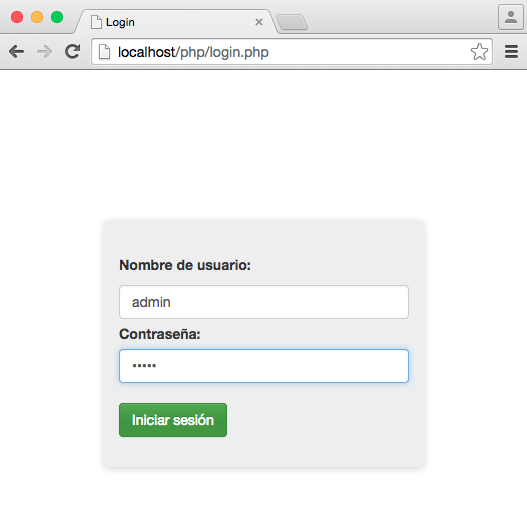
\includegraphics[scale=0.50]{images/capitulo6/rfq001.png}}
\caption{RFQ-001 Ventana Inicio sesión.}
\label{rfq001}
\end{figure}

Después de presionar el botón: "Iniciar sesión" se abrirá la página principal con acceso a todas las funcionalidades del sistema. Ver Figura 62.

\begin{figure}[H]
\centering
\setlength\fboxsep{0pt}
\setlength\fboxrule{0.5pt}
\fbox{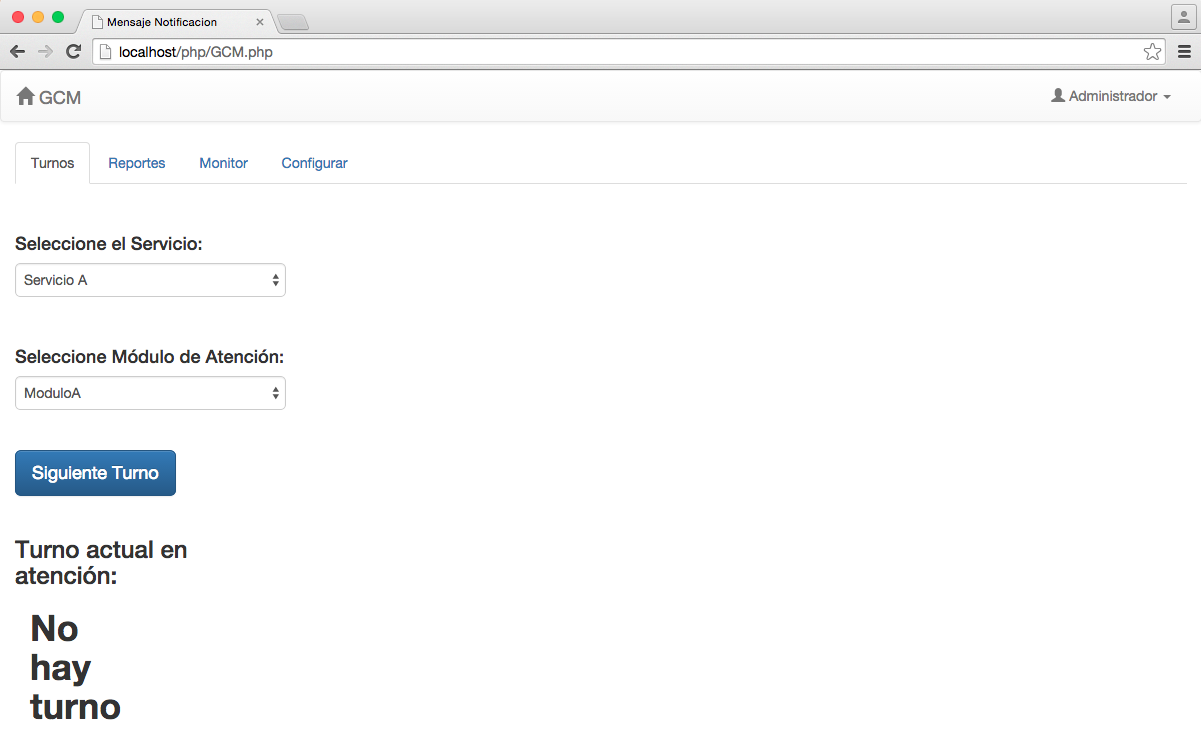
\includegraphics[scale=0.30]{images/capitulo6/rfq001a.png}}
\caption{RFQ-001 Ventana principal aplicación web.}
\label{rfq001}
\end{figure}


\subsubsection{RFQ - 002 Cargar y mostrar servicios.}

El combobox que se aprecia en la Figura 63, contiene los servicios que provee el sistema, estos datos son traídos desde base de datos. Por ejemplo, corresponde a los servicios que entregaría el centro de atención donde se implemente el sistema de gestión de tickets.\\ 

\begin{figure}[H]
\centering
\setlength\fboxsep{0pt}
\setlength\fboxrule{0.5pt}
\fbox{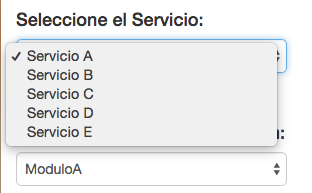
\includegraphics[scale=0.60]{images/capitulo6/rfq002.png}}
\caption{RFQ-002 Combobox con servicios.}
\label{rfq002}
\end{figure}

\subsubsection{RFQ - 003 Cargar y mostrar módulos de atención.}

Este requisito es similar al anterior. En la Figura 64 se exhiben, los datos cargados desde la base de datos, los módulos de atención que están prestando un servicio en el centro de atención.

\begin{figure}[H]
\centering
\setlength\fboxsep{0pt}
\setlength\fboxrule{0.5pt}
\fbox{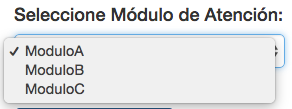
\includegraphics[scale=0.60]{images/capitulo6/rfq003.png}}
\caption{RFQ-003 Combobox con módulos de atención.}
\label{rfq003}
\end{figure}

\subsubsection{RFQ - 004 Enviar notificaciones desde aplicación web a \textit{smartphone}.}

Este botón, Figura 65, utiliza los dos requisitos anteriores (RFQ-001 y RFQ-002). Se encarga de enviar notificaciones exclusivamente a los dispositivos que han tomado un ticket de atención en el servicio que esté seleccionado en RFQ-001. También se envía el nombre del módulo, que será mostrado en el dispositivo móvil cuando sea el turno del cliente y pueda saber a qué módulo de atención debe pasar para ser atendido.

\begin{figure}[H]
\centering
\setlength\fboxsep{0pt}
\setlength\fboxrule{0.5pt}
\fbox{
\includegraphics[scale=0.60]{images/capitulo6/rfq005.png}}
\caption{RFQ-004 Botón para enviar notificaciones.}
\label{rfq005}
\end{figure}


\subsubsection{RFQ - 005  Generar reportes.}

Los reportes se generan automáticamente al hacer click en la pestaña "Reportes". Utilizan los datos almacenados en la base de datos. Se dispone de un gráfico de barras y uno de líneas. El primero, Figura 66, muestra un resumen del número de atenciones que ha tenido cada servicio el último año. El segundo, Figura 67, corresponde al detalle de la cantidad de atenciones que ha tenido cada servicio mensualmente el último año.

\begin{figure}[H]
\centering
\setlength\fboxsep{0pt}
\setlength\fboxrule{0.5pt}
\fbox{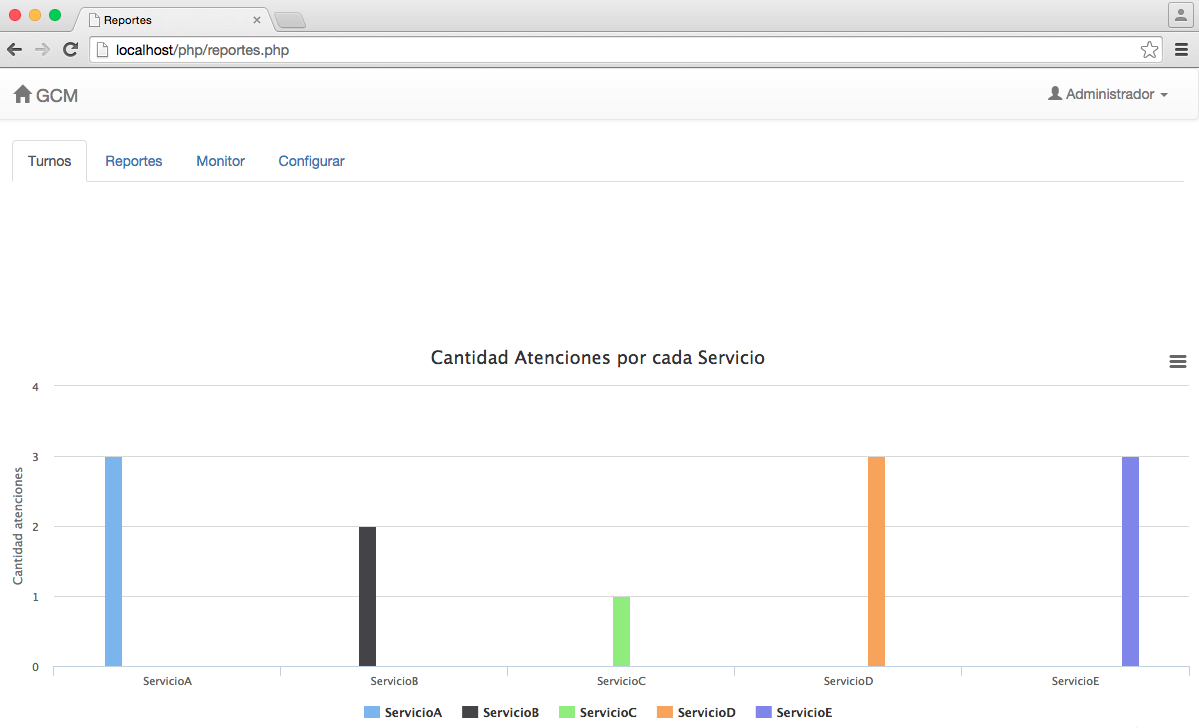
\includegraphics[scale=0.30]{images/capitulo6/rfq004a.png}}
\caption{RFQ-004 Gráfico barra número de atenciones por servicio.}
\label{rfq004}
\end{figure}

\begin{figure}[H]
\centering
\setlength\fboxsep{0pt}
\setlength\fboxrule{0.5pt}
\fbox{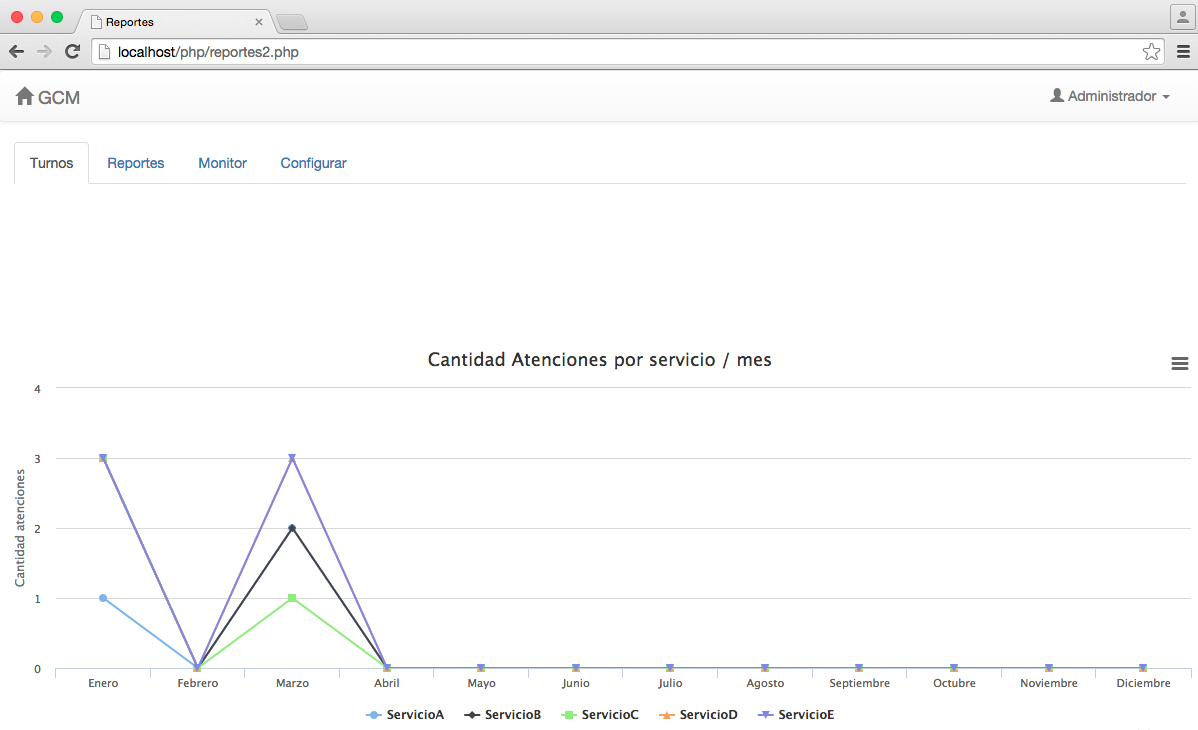
\includegraphics[scale=0.30]{images/capitulo6/rfq004b.png}}
\caption{RFQ-004 Gráfico líneas número de atenciones al mes.}
\label{rfq004}
\end{figure}

\subsubsection{RFQ - 006 Mostrar últimos turnos en atención.}

Al final de la ventana en la figura 68, se aprecia la etiqueta "Turno actual en atención:". Bajo ésta, se entrega el número de ticket que está siendo atendido correspondiente al servicio que está seleccionado, RFQ-001.

\begin{figure}[H]
\centering
\setlength\fboxsep{0pt}
\setlength\fboxrule{0.5pt}
\fbox{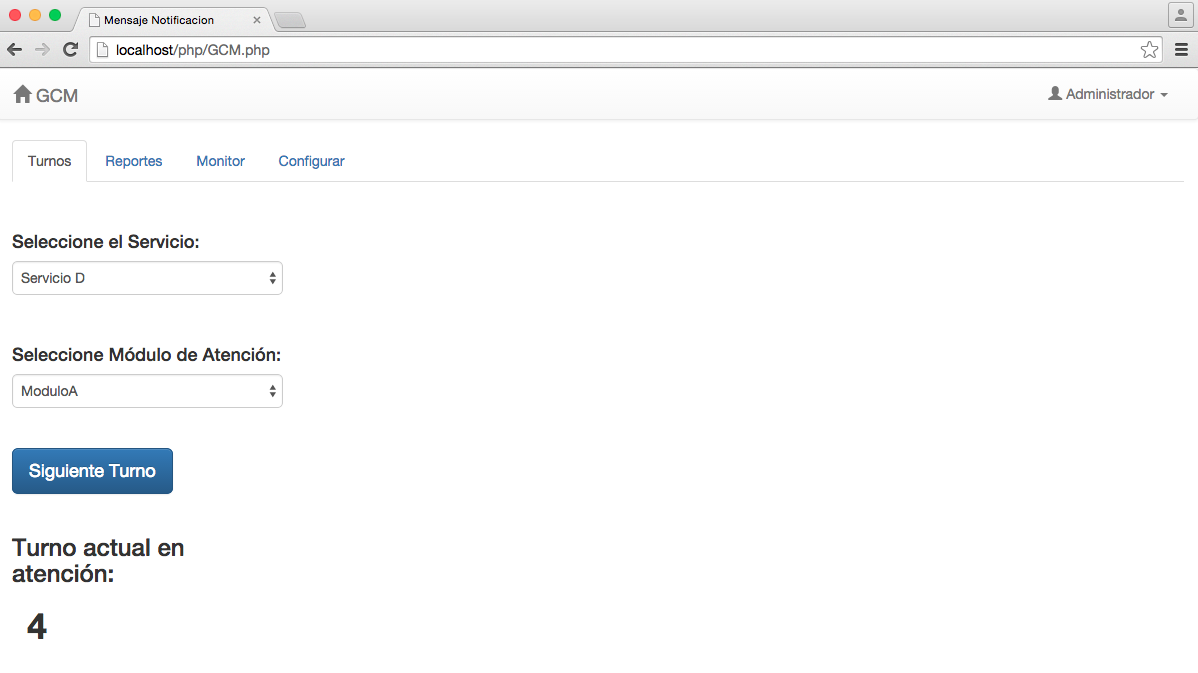
\includegraphics[scale=0.30]{images/capitulo6/rfq006.png}}
\caption{RFQ-006 Turno en atención correspondiente al Servicio D.}
\label{rfq006}
\end{figure}

\subsubsection{RFQ - 007 Monitor de atenciones.}

El monitor de atenciones, Figura 69, cumple las funciones de informar a los clientes, que están esperando en el centro de atención, a qué módulo de atención deben pasar. para ello, se muestra el número de turno y el tipo de servicio.

\begin{figure}[H]
\centering
\setlength\fboxsep{0pt}
\setlength\fboxrule{0.5pt}
\fbox{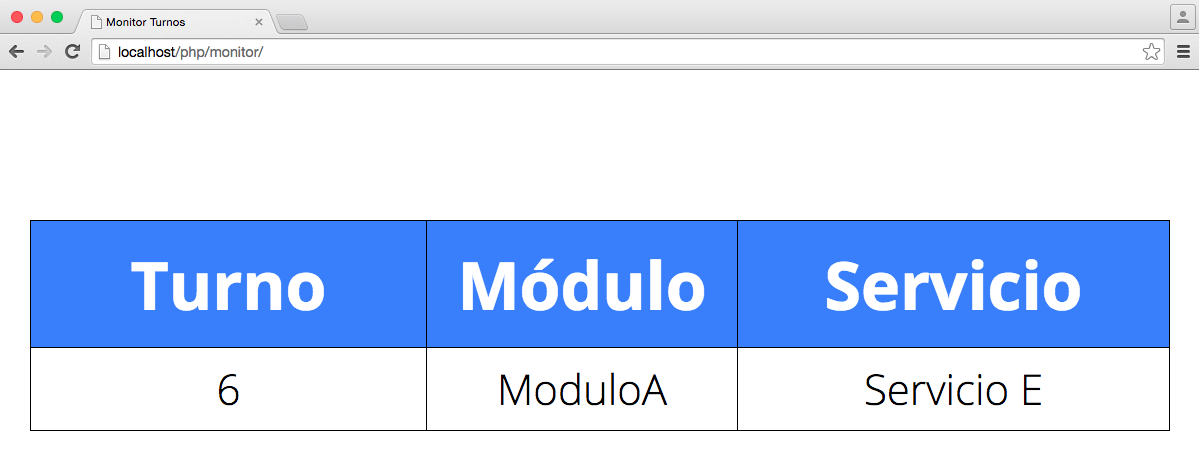
\includegraphics[scale=0.30]{images/capitulo6/rfq007.png}}
\caption{RFQ-007 Monitor muestra turno, módulo y servicio.}
\label{rfq007}
\end{figure}


\subsection{Prueba de Aplicación móvil.}

El orden de las siguientes pruebas obedecen a la Tabla 3. Requisitos funcionales, desde el RFQ 008 - 013.\\

En el ítem anterior, 5.3.4 Aplicación Móvil, ya se explicó lo que muestra la aplicación móvil. La diferencia es que acá se hace énfasis en el cumplimiento de los requisitos funcionales. A continuación se muestra la secuencia normal que surge al utilizar la aplicación móvil para solicitar un ticket de atención, Figuras: 70, 71, 72, 73, 74. 

\subsubsection{RFQ - 008 Mostrar servicios.}

\begin{figure}[H]
\centering
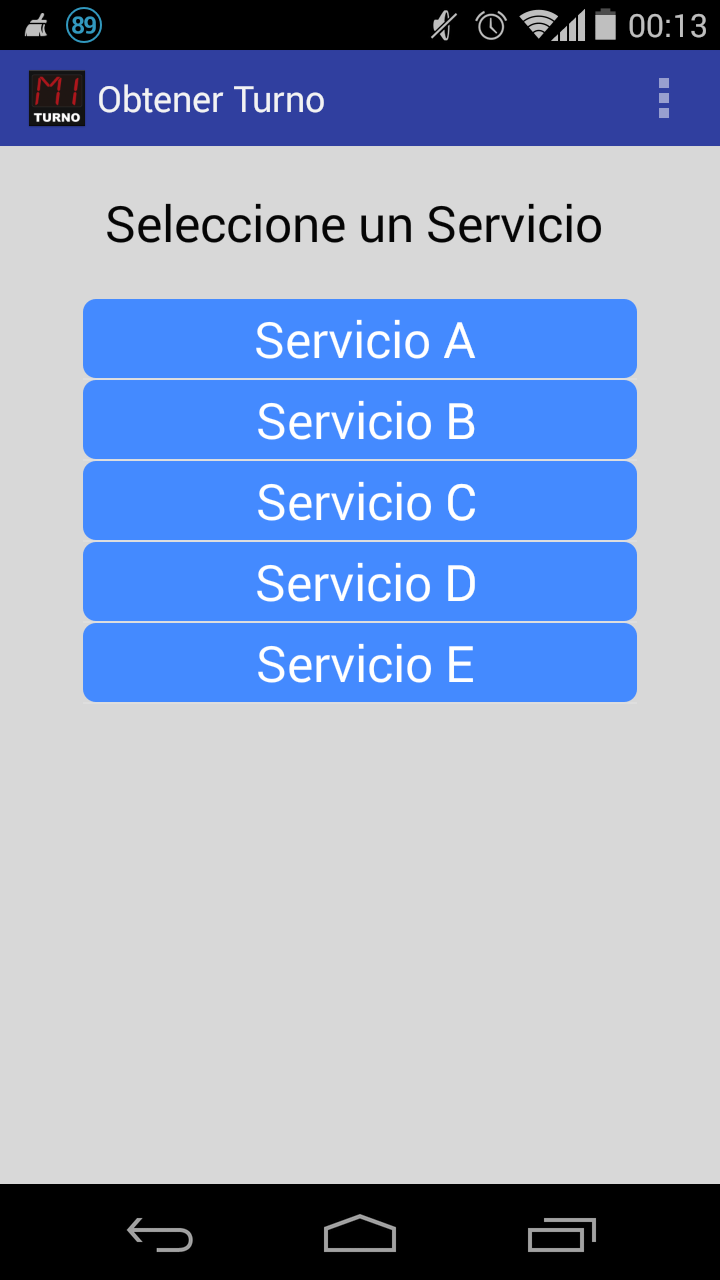
\includegraphics[scale=0.20]{images/capitulo6/rfq008.png}
\caption{RFQ-008 Servicios disponibles.}
\label{rfq008}
\end{figure}

\subsubsection{RFQ - 009 Seleccionar un servicio.}

\begin{figure}[H]
\centering
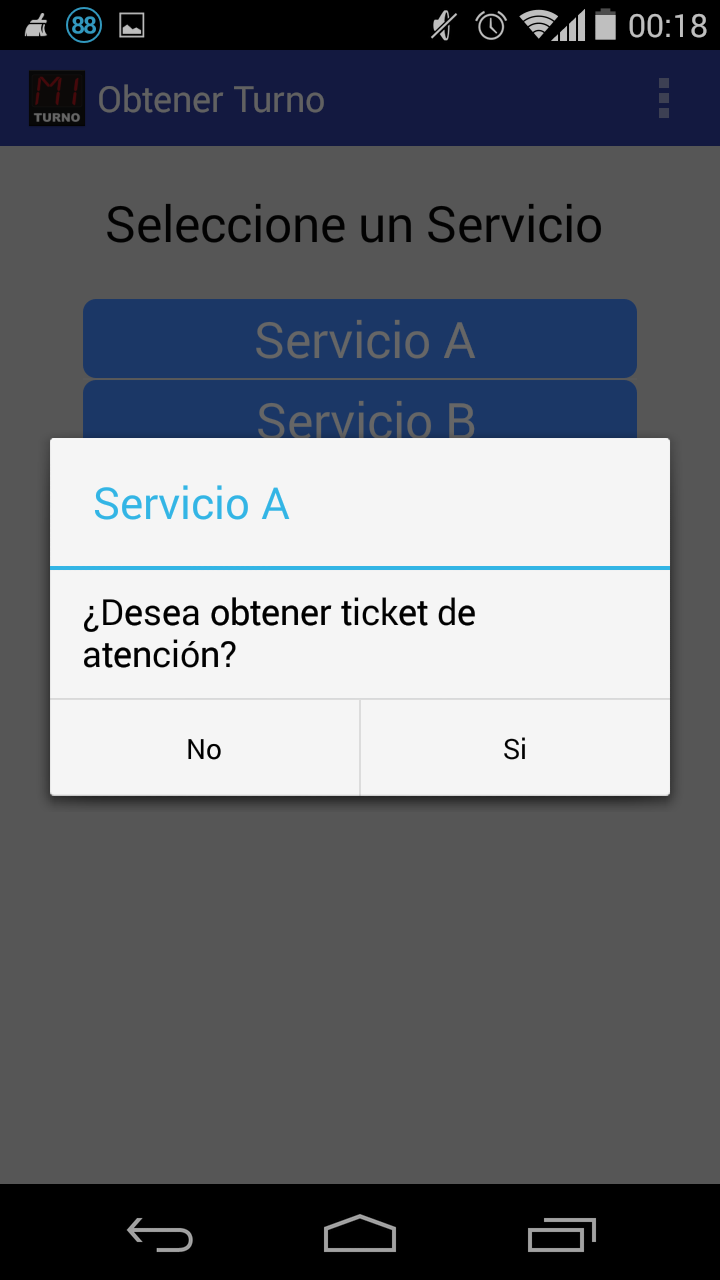
\includegraphics[scale=0.20]{images/capitulo6/rfq009.png}
\caption{RFQ-009 Selección de Servicio A.}
\label{rfq009}
\end{figure}

\subsubsection{RFQ - 010 Ver turno de atención.}

\begin{figure}[H]
\centering
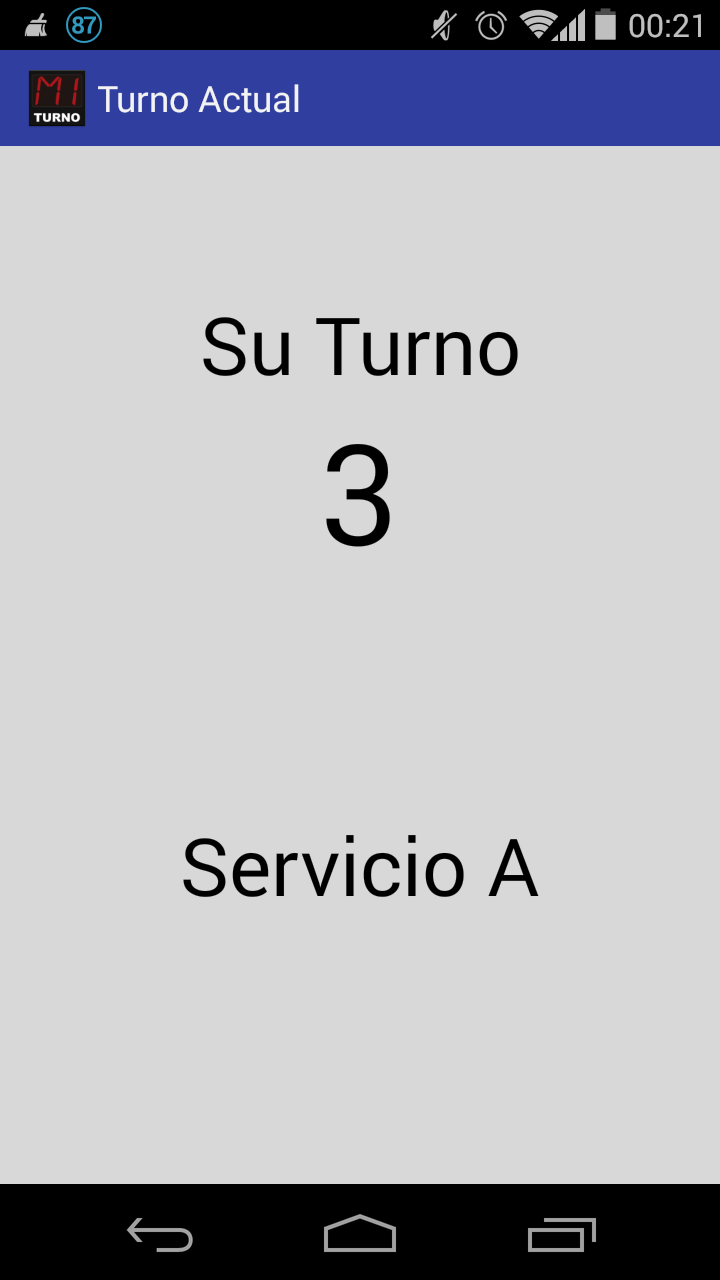
\includegraphics[scale=0.20]{images/capitulo6/rfq010.png}
\caption{RFQ-010 Turno de atención obtenido.}
\label{rfq010}
\end{figure}

\subsubsection{RFQ - 011 Ver notificaciones.}

\begin{figure}[H]
\centering
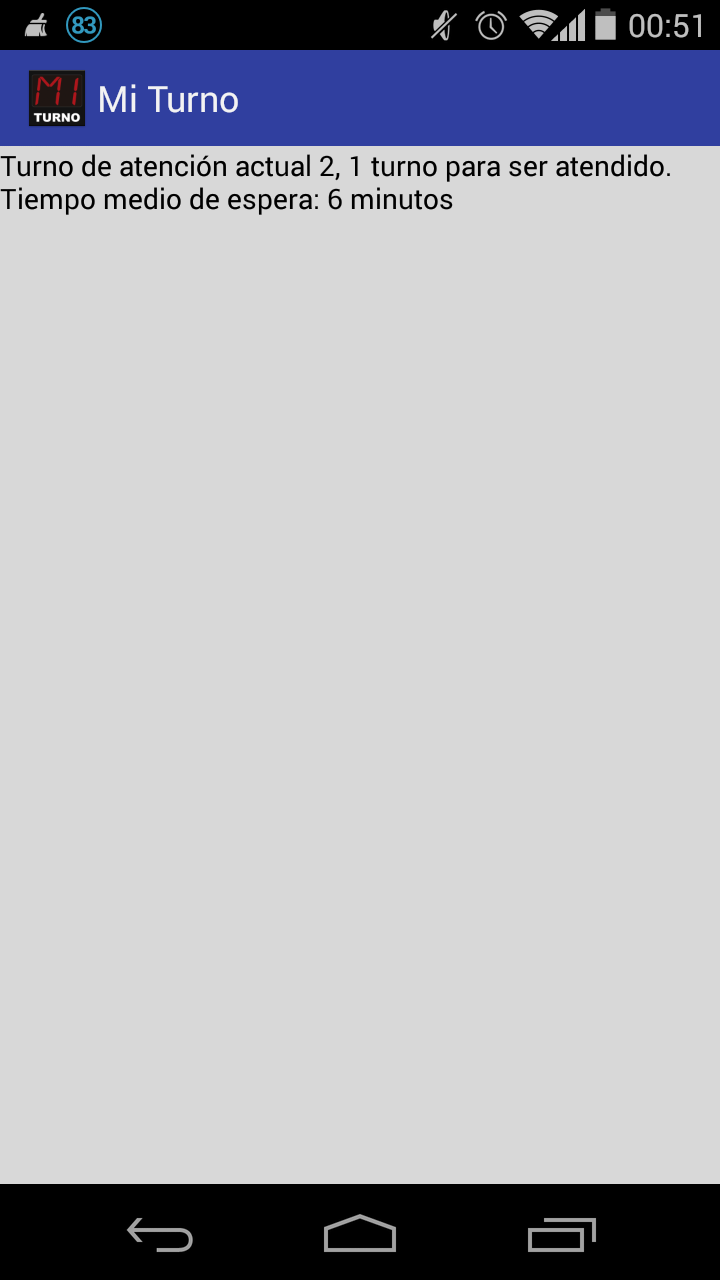
\includegraphics[scale=0.20]{images/capitulo6/rfq011.png}
\caption{RFQ-011 Notificación recibida desde aplicación web.}
\label{rfq011}
\end{figure}

\subsubsection{RFQ - 012 Mostrar notificaciones nuevas automáticamente.}

\begin{figure}[H]
\centering
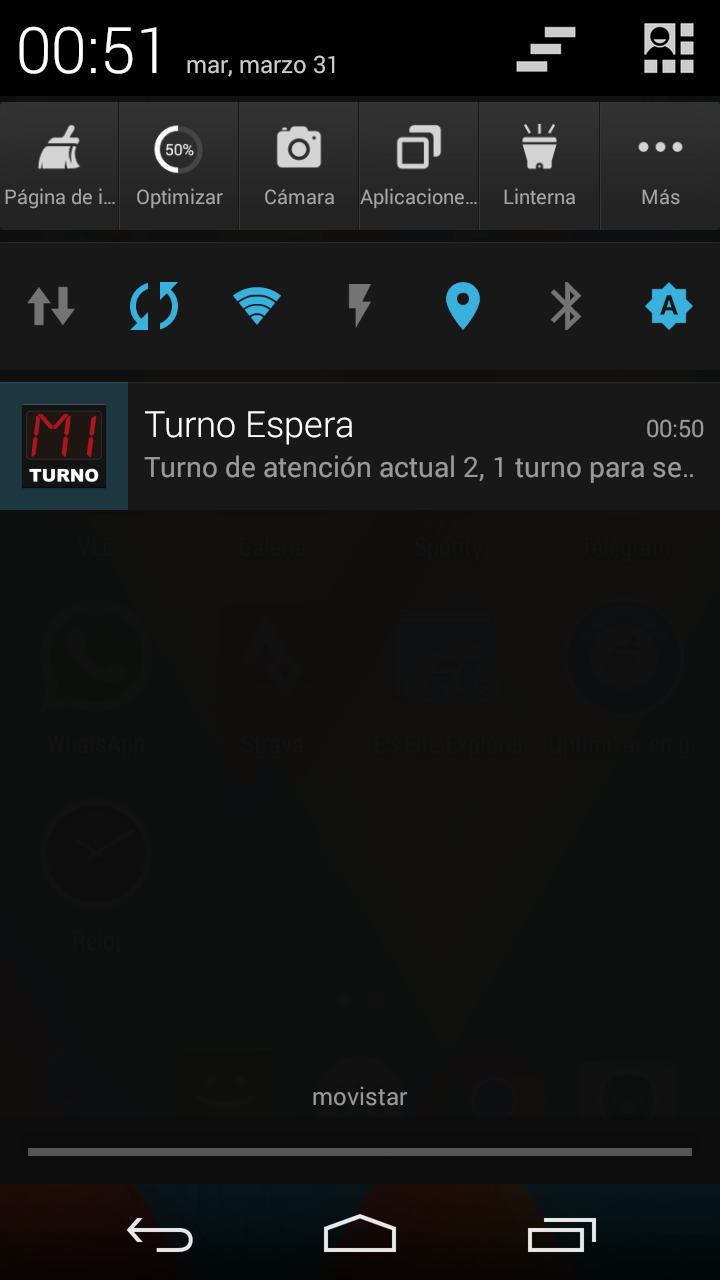
\includegraphics[scale=0.20]{images/capitulo6/rfq012.png}
\caption{RFQ-012 Notificación Push.}
\label{rfq012}
\end{figure}

\subsubsection{RFQ - 013 Mostrar información de la aplicación.}

\begin{figure}[H]
\centering
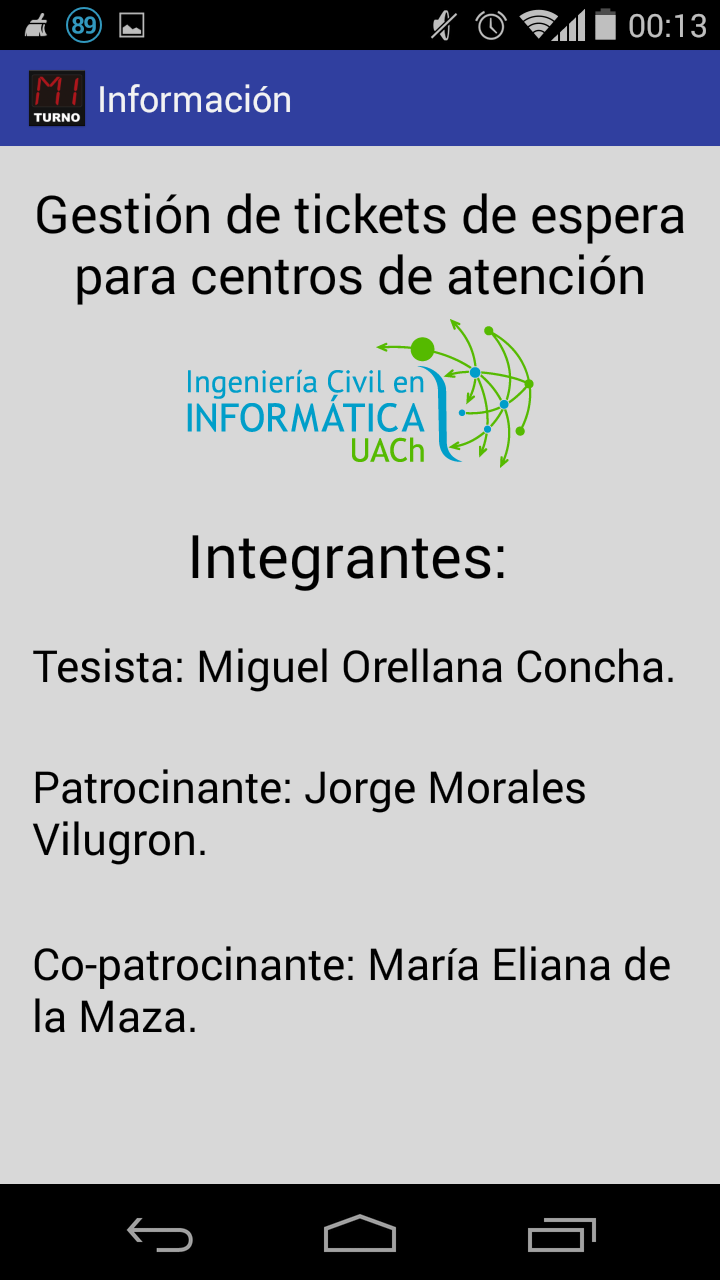
\includegraphics[scale=0.20]{images/capitulo6/rfq013.png}
\caption{RFQ-013 Información del proyecto.}
\label{rfq013}
\end{figure}

